%
% Copyright 2018 Joel Feldman, Andrew Rechnitzer and Elyse Yeager.
% This work is licensed under a Creative Commons Attribution-NonCommercial-ShareAlike 4.0 International License.
% https://creativecommons.org/licenses/by-nc-sa/4.0/
%
\questionheader{ex:s1.5}

%%%%%%%%%%%%%%%%%%
\subsection*{\Conceptual}
%%%%%%%%%%%%%%%%%%
\begin{question}
We want to approximate the area between the graphs of $y=\cos x$ and $y=\sin x$ from $x=0$ to $x=\pi$ using a left Riemann sum with $n=4$ rectangles.
\begin{enumerate}[(a)]
\item On the graph below, sketch the four rectangles.
\item Calculate the Riemann approximation.
\end{enumerate}
\begin{center}
\begin{tikzpicture}
\YEaaxis{1}{4.5}{2}{2.25};
\YExcoord{3.14}{\pi}
\YExcoord{1.57}{\frac{\pi}{2}}
\YExcoord{0.79}{\frac{\pi}{4}}
\YExcoord{2.36}{\frac{3\pi}{4}}
\draw[blue, thick] plot[domain=-.5:3.7](\x,{2*cos(\x r)}) node[right]{$y=\cos x$};
\draw[black, thick] plot[domain=-.5:3.7](\x,{2*sin(\x r)}) node[right]{$y=\sin x$};
\end{tikzpicture}
\end{center}
\end{question}
\begin{hint}
When we say ``area between," we want positive area, \emph{not} signed area.
\end{hint}
\begin{answer}
Area between curves $\approx \frac{\pi}{4}\left(2+\sqrt{2}\right)$

\begin{tikzpicture}
\YEaaxis{1}{4.5}{2}{2.25};
\YExcoord{3.14}{\pi}
\YExcoord{1.57}{\frac{\pi}{2}}
\YExcoord{0.79}{\frac{\pi}{4}}
\YExcoord{2.36}{\frac{3\pi}{4}}
\draw[blue, thick] plot[domain=-.5:3.7](\x,{2*cos(\x r)}) node[right]{$y=\cos x$};
\draw[black, thick] plot[domain=-.5:3.7](\x,{2*sin(\x r)}) node[right]{$y=\sin x$};
\draw[red, fill=red, fill opacity=0.5] (0,0) rectangle (0.79,2)
(0.79,1.41) -- (1.57,1.41)
(1.57,0) rectangle(2.36,2)
(2.36,-1.41) rectangle (3.14,1.41);
\end{tikzpicture}
\end{answer}
\begin{solution}
\begin{center}
\begin{tikzpicture}
\YEaaxis{1}{4.5}{2}{2.25};
\YExcoord{3.14}{\pi}
\YExcoord{1.57}{\frac{\pi}{2}}
\YExcoord{0.79}{\frac{\pi}{4}}
\YExcoord{2.36}{\frac{3\pi}{4}}
\draw[blue, thick] plot[domain=-.5:3.7](\x,{2*cos(\x r)}) node[right]{$y=\cos x$};
\draw[black, thick] plot[domain=-.5:3.7](\x,{2*sin(\x r)}) node[right]{$y=\sin x$};
\draw[red, fill=red, fill opacity=0.5] (0,0) rectangle (0.79,2)
(0.79,1.41) -- (1.57,1.41)
(1.57,0) rectangle(2.36,2)
(2.36,-1.41) rectangle (3.14,1.41);
\end{tikzpicture}
\end{center}
The intervals of our rectangles are $[0,\frac{\pi}{4}]$, $[\frac{\pi}{4},\frac{\pi}{2}]$,
$[\frac{\pi}{2},\frac{3\pi}{4}]$, and $[\frac{3\pi}{4},\pi]$. Since we're taking a left Riemann sum, we find the height of the rectangles at the left endpoints of the intervals.
\begin{description}
\item[$x = 0$:] The distance from $\cos 0$ to $\sin 0$ is 1, so our first rectangle has height 1.
\item[$x = \frac{\pi}{4}$:] The distance from $\cos \frac{\pi}{4}$ to $\sin \frac{\pi}{4}$ is 0, so our second rectangle has height 0.
\item[$x = \frac{\pi}{2}$:] The distance from $\cos \frac{\pi}{2}$ to $\sin \frac{\pi}{2}$ is 1, so our third rectangle has height 1.
\item[$x = \frac{3\pi}{4}$:] The distance from $\cos \frac{3\pi}{4}$ to $\sin \frac{3\pi}{4}$ is $\sin(3\pi/4)-\cos(3\pi/4) =\frac{1}{\sqrt{2}}-\left(-\frac{1}{\sqrt{2}}\right)=\sqrt{2} $, so our fourth rectangle has height $\sqrt{2}$.
\end{description}
So, our approximation for the area between the two curves is
\[\frac{\pi}{4}\left(1+0+1+\sqrt{2}\right)=\frac{\pi}{4}\left(2+\sqrt{2}\right)\]
\end{solution}
%%%%%%%%%%%%%%%%%%%
\begin{question}
We want to approximate the bounded area between the curves $y=\arcsin\left(\dfrac{2x}{\pi}\right)$ and $y=\sqrt{\dfrac{\pi x}{2}}$ using $n=5$ rectangles.
\begin{enumerate}[(a)]
\item Draw the five (vertical) rectangles on the picture below corresponding to a right Riemann sum.
\item Draw  five rectangles on the picture below we might use if we were using horizontal rectangles.
\end{enumerate}
\begin{center}
\begin{tikzpicture}
\YEaaxis{1.5}{7}{1.5}{6}
\YExcoord{6.28}{\frac{\pi}{2}}
\draw[thick, blue] plot[domain=-.2:1.57, xscale=4, yscale=4]({sin(\x r)/2*3.14},{\x}) ;
\draw[blue] (4,1)node{$y=\arcsin\left(\frac{2x}{\pi}\right)$};
\draw[thick] plot[domain=0:1.8, xscale=4, yscale=4, samples=100]({\x},{sqrt(\x*3.14/2)});
\draw (2,4.75)node{$y=\sqrt{\frac{x\pi}{2}}$};
\end{tikzpicture}
\end{center}
\end{question}
\begin{hint}
We're taking rectangles that reach from one function to the other.
\end{hint}
\begin{answer}
(a) Vertical rectangles:\\
\begin{tikzpicture}
\YEaaxis{1.5}{7}{1.5}{6}
\foreach \x/\l in {1.26/\frac{\pi}{10},2.51/\frac{\pi}{5},3.77/\frac{3\pi}{10},5.03/\frac{2\pi}{5},6.28/\frac{\pi}{2}}
 	{\YExcoord{\x}{\l}}
\draw[red, fill=red, fill opacity=0.5]
 (0,0.8)rectangle (1.26,2.81)
  (1.26,1.64)rectangle (2.51,3.97)
   (2.51,2.56)rectangle (3.77,4.87)
    (3.77,3.72)rectangle (5.03,5.62)
        (5.03,6.28)rectangle (6.28,6.28);
\draw[thick, blue] plot[domain=-.2:1.57, xscale=4, yscale=4]({sin(\x r)/2*3.14},{\x}) ;
\draw[blue] (4,1)node{$y=\arcsin\left(\frac{2x}{\pi}\right)$};
\draw[thick] plot[domain=0:1.8, xscale=4, yscale=4, samples=100]({\x},{sqrt(\x*3.14/2)});
\draw (2,5.25)node{$y=\sqrt{\frac{x\pi}{2}}$};
\end{tikzpicture}

(b) One possible answer:\\
\begin{tikzpicture}
\YEaaxis{1.5}{7}{1.5}{7}
\foreach \x/\l in {1.26/\frac{\pi}{10},2.51/\frac{\pi}{5},3.77/\frac{3\pi}{10},5.03/\frac{2\pi}{5},6.28/\frac{\pi}{2}}
 	{\YEycoord{\x}{\l});}
\draw[red, fill=red, fill opacity=0.5]
 (1.94,0)rectangle (0.25,1.26)
  (3.69,1.26)rectangle (1,2.51)
   (5.08,2.51)rectangle (2.26,3.77)
    (5.98,3.77)rectangle (4.02,5.03)
        (6.28,5.03)rectangle (6.28,6.28);
\draw[thick, blue] plot[domain=-.2:1.57, xscale=4, yscale=4]({sin(\x r)/2*3.14},{\x}) ;
\draw[blue] (4,1)node{$x=\frac{\pi}{2}\sin y$};
\draw[thick] plot[domain=0:1.8, xscale=4, yscale=4, samples=100]({\x},{sqrt(\x*3.14/2)});
\draw (2,5.25)node{$x=\frac{2}{\pi}y^2$};
\end{tikzpicture}


\end{answer}
\begin{solution}

\begin{enumerate}[(a)]
\item We are finding the area in the interval from $x=0$ to $x=\frac{\pi}{2}$. Since we're taking $n=5$ rectangles, our rectangles cover the following intervals:
\[
\left[0,\frac{\pi}{10}\right],\quad
\left[\frac{\pi}{10},\frac{\pi}{5}\right],\quad
\left[\frac{\pi}{5},\frac{3\pi}{10}\right],\quad
\left[\frac{3\pi}{10},\frac{2\pi}{5}\right],\quad
\left[\frac{2\pi}{5},\frac{\pi}{2}\right].\]

\begin{center}
\begin{tikzpicture}
\YEaaxis{1.5}{7}{1.5}{6}
\foreach \x/\l in {1.26/\frac{\pi}{10},2.51/\frac{\pi}{5},3.77/\frac{3\pi}{10},5.03/\frac{2\pi}{5},6.28/\frac{\pi}{2}}
 	{\YExcoord{\x}{\l}}
\draw[red, fill=red, fill opacity=0.5]
 (0,0.8)rectangle (1.26,2.81)
  (1.26,1.64)rectangle (2.51,3.97)
   (2.51,2.56)rectangle (3.77,4.87)
    (3.77,3.72)rectangle (5.03,5.62)
        (5.03,6.28)rectangle (6.28,6.28);
\draw[thick, blue] plot[domain=-.2:1.57, xscale=4, yscale=4]({sin(\x r)/2*3.14},{\x}) ;
\draw[blue] (4,1)node{$y=\arcsin\left(\frac{2x}{\pi}\right)$};
\draw[thick] plot[domain=0:1.8, xscale=4, yscale=4, samples=100]({\x},{sqrt(\x*3.14/2)});
\draw (2,5.25)node{$y=\sqrt{\frac{x\pi}{2}}$};
\end{tikzpicture}
\end{center}

\item We are finding the area in the interval from $y=0$ to $y=\frac{\pi}{2}$. (In general, when we switch from horizontal rectangles to vertical, the limits of integration will change--it's only coincidence that they are the same in this example.) Since we're taking $n=5$ rectangles, these rectangles cover the following intervals of the $y$-axis:
\[
\left[0,\frac{\pi}{10}\right],\quad
\left[\frac{\pi}{10},\frac{\pi}{5}\right],\quad
\left[\frac{\pi}{5},\frac{3\pi}{10}\right],\quad
\left[\frac{3\pi}{10},\frac{2\pi}{5}\right],\quad
\left[\frac{2\pi}{5},\frac{\pi}{2}\right].\]

The question doesn't specify which endpoints we're using. Let's use upper endpoints, to match part (a).

\begin{center}
\begin{tikzpicture}
\YEaaxis{1.5}{7}{1.5}{7}
\foreach \x/\l in {1.26/\frac{\pi}{10},2.51/\frac{\pi}{5},3.77/\frac{3\pi}{10},5.03/\frac{2\pi}{5},6.28/\frac{\pi}{2}}
 	{\YEycoord{\x}{\l});}
\draw[red, fill=red, fill opacity=0.5]
 (1.94,0)rectangle (0.25,1.26)
  (3.69,1.26)rectangle (1,2.51)
   (5.08,2.51)rectangle (2.26,3.77)
    (5.98,3.77)rectangle (4.02,5.03)
        (6.28,5.03)rectangle (6.28,6.28);
\draw[thick, blue] plot[domain=-.2:1.57, xscale=4, yscale=4]({sin(\x r)/2*3.14},{\x}) ;
\draw[blue] (4,1)node{$x=\frac{\pi}{2}\sin y$};
\draw[thick] plot[domain=0:1.8, xscale=4, yscale=4, samples=100]({\x},{sqrt(\x*3.14/2)});
\draw (2,5.25)node{$x=\frac{2}{\pi}y^2$};
\end{tikzpicture}
\end{center}

\end{enumerate}
\end{solution}
%%%%%%%%%%%%%%%%%%%


\begin{Mquestion}[M121 2002A]
Write down a definite integral that represents the
finite area bounded by the curves $y=x^3-x$ and
$y=x$ for $x\ge 0$.
\emph{Do not evaluate the integral explicitly.}
\end{Mquestion}

\begin{hint}
Draw a sketch first.
\end{hint}

\begin{answer}
$ \displaystyle\int_0^{\sqrt{2}}\big[2x-x^3\big]\ \dee{x}$
\end{answer}

\begin{solution}
The curves intersect when $y=x$ and $y=x^3-x$. To find these points, we set:
\begin{align*}
x&=x^3-x\\
0&=x^3-2x\\
0&=x(x^2-2)\\
0&= x \quad\mbox{or}\quad 0=x^2-2
\end{align*}
For $x\ge 0$, the curves intersect at $(0,0)$ and $(\sqrt{2},\sqrt{2})$.

A handy observation is that, since both curves are continuous and they do not meet each other between $x=0$ and $x=\sqrt{2}$, we don't have to worry about dividing our area into two regions: one of the functions is always on the top, and the other is always on the bottom.

Using vertical strips:
\begin{center}
       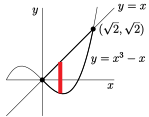
\includegraphics{OE02A_2a}
\end{center}
The top and bottom boundaries of the specified region are $y=T(x)=x$
and $y=B(x)=x^3-x$, respectively. So,
\begin{align*}
{\rm Area} = \int_0^{\sqrt{2}}\big[T(x)-B(x)\big]\ \dee{x}
= \int_0^{\sqrt{2}}\big[x-(x^3-x)\big]\ \dee{x} = \int_0^{\sqrt{2}} 2x-x^3 \ \dee{x}
\end{align*}

\end{solution}
%%%%%%%%%%%%%%%%%%%%%%%%%%%%%%%%%%%%%%%%


\begin{question}[2000D]
Write down a definite integral that represents the
area of the region bounded by the line $y=-\dfrac{x}{2}$
and the parabola $y^2=6-\dfrac{5x}{4}$.
\emph{Do not evaluate the integral explicitly.}
\end{question}


\begin{hint}
Draw a sketch first.
\end{hint}

\begin{answer}
$\displaystyle \int_{-3/2}^{4}\left[\frac{4}{5}(6-y^2)+2y\right]\ \dee{y}$
\end{answer}

\begin{solution}
We need to find where the curves intersect.
\begin{align*}
\frac{x^2}{4}=y^2&=6-\dfrac{5x}{4}\\
\frac{1}{4}x^2+\frac{5}{4}x-6&=0\\
x^2+5x-24&=0\\
(x+8)(x-3)&=0\\
x=-8,\quad x&=3
\end{align*}

The curves intersect at $(-8,4)$ and $(3,-\frac{3}{2})$.  Using horizontal
strips:
\begin{center}
       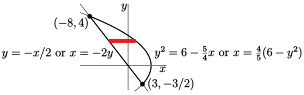
\includegraphics{OE00D_3a}
\end{center}
we have
\begin{align*}
\text{Area} = \int_{-3/2}^{4}\Big[\frac{4}{5}(6-y^2)+2y\Big]\ \dee{y}
\end{align*}

\end{solution}
%%%%%%%%%%%%%%%%%%%%%%%%%%%%%%%%%%%%%%%%


\begin{question}[2001A]\label{1.5_4ax4ay}
Write down a definite integral that represents the
area of the finite plane region bounded by $y^2=4ax$ and
$x^2=4ay$, where $a>0$ is a constant.
\emph{Do not evaluate the integral explicitly.}
\end{question}

\begin{hint}
You can probably find the intersections by inspection.
\end{hint}

\begin{answer}
$ \displaystyle\int_0^{4a}\left[\sqrt{4ax}-\frac{x^2}{4a}\right]\ \dee{x}$
\end{answer}

\begin{solution}
If the curves intersect at $(x,y)$, then
\begin{align*}
\left(x^2\right)^2&=\left(4a\right)^2y^2 = (4a)^24ax\\
x^4&=(4a)^3 x\\
x^4&-(4a)^3x=0\\
x(&x^3-(4a)^3)=0\\
x&= 0 \quad\mbox{or}\quad x^3=(4a)^3
\end{align*}
The curves intersect at $(0,0)$ and $(4a,4a)$. (It is also possible to find these points by inspection.) Using vertical strips:
\begin{center}
       
\includegraphics{OE01A_2a}
\end{center}
We want the $y$-values of the functions. We write the top  function as $y =\sqrt{4ax}$ (we care about the positive square root, not the negative one) and we write the bottom function as $y=\frac{x^2}{4a}$.
Then we have
\begin{align*}
\text{Area} = \int_0^{4a}\left[\sqrt{4ax}-\frac{x^2}{4a}\right]\ \dee{x}
\end{align*}

\end{solution}
%%%%%%%%%%%%%%%%%%%%%%%%%%%%%%%%%%%%%%%%

\begin{Mquestion}[2001D]
Write down a definite integral that represents the
area of the region bounded between the line $x+12y+5=0$
and the curve  $x=4y^2$.
\emph{Do not evaluate the integral explicitly.}
\end{Mquestion}

\begin{hint}
To find the intersection, plug $x=4y^2$ into the equation $x+12y+5=0$.
\end{hint}

\begin{answer}
$\displaystyle\int_1^{25}\left[-\frac{1}{12}(x+5)+\frac{1}{2}\sqrt{x}\right]\ \dee{x}$
\end{answer}

\begin{solution}
The curves intersect when $x=4y^2$ and $0=4y^2+12y+5
=(2y+5)(2y+1)$. So, the curves intersect at $(1,-\half)$ and $(25,-\frac{5}{2})$.
Using vertical strips:
\begin{center}
       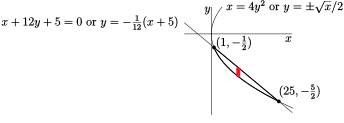
\includegraphics{OE01D_3a}
\end{center}
we have
\begin{align*}
\text{Area} =
\int_1^{25}\left[-\frac{1}{12}(x+5)+\frac{1}{2}\sqrt{x}\right]\ \dee{x}
\end{align*}

\end{solution}
%%%%%%%%%%%%%%%%%%%%%%%%%%%%%%%%%%%%%%%%



%%%%%%%%%%%%%%%%%%
\subsection*{\Procedural}
%%%%%%%%%%%%%%%%%%



\begin{Mquestion}[M105 2013A]
Find the area of the region bounded by the graph of
$f (x) = \dfrac{1}{(2x-4)^2}$ and the $x$--axis
between $x = 0$ and $x = 1$.
\end{Mquestion}

\begin{hint}
If the bottom function is the $x$-axis, this is a familiar question.
\end{hint}

\begin{answer}
$\dfrac{1}{8}$
\end{answer}

\begin{solution}
\begin{center}
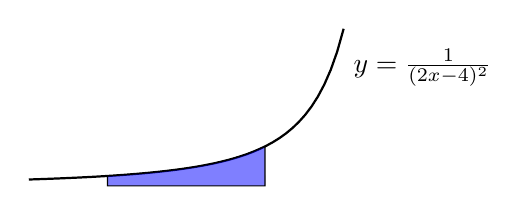
\begin{tikzpicture}
\YEaaxis{1}{3.5}{1}{2}
\YExcoord{2}{1}
\draw[thick] plot[domain=-.5:1.5, samples=50, scale=2](\x,{1/(4*(\x-2)*(\x-2))});
\draw[fill=blue, fill opacity=0.5] plot[domain=0:1, samples=10, scale=2](\x,{1/(4*(\x-2)*(\x-2))})--(2,0)-|cycle;
\draw (3,1.5)node[right]{$y=\frac{1}{(2x-4)^2}$};
\end{tikzpicture}
\end{center}

The area between the curve $y= \frac{1}{(2x-4)^2}$
and the $x$-axis, with $x$ running from $a=0$ to
$b=1$, is exactly the definite integral of $\frac{1}{(2x+4)^2}$ with limits $0$ and $1$.

\begin{align*}
\mbox{Area}&=\int_0^1 \frac{\dee{x}}{(2x-4)^2}&u=2x-4,\quad\dee{u}=2\ \dee{x}\\
&=\frac{1}{2}\int_{-4}^{-2}\frac{1}{u^2}\dee{u} = \frac{1}{2}\left[\frac{-1}{u}\right]_{u=-4}^{u=-2}\\
&=\frac{1}{2}\Big[\frac{1}{2}-\frac{1}{4}\Big]
=\frac{1}{8}
\end{align*}

\end{solution}
%%%%%%%%%%%%%%%%%%%

\begin{question}[2016Q2]
Find the area between the curves $y=x$ and $y=3x-x^2$, by first identifying the points of intersection and then integrating.
\end{question}

\begin{hint}
Part of the job is to determine whether $y=x$ lies above or below
$y=3x-x^2$.
\end{hint}

\begin{answer}
$\dfrac{4}{3}$
\end{answer}

\begin{solution}
If the curves $y=f(x)=x$ and $y=g(x)=3x-x^2$ intersect at $(x,y)$, then
\begin{align*}
3x-x^2&=y=x\\
x^2-2x&=0\\
x(x-2)&=0\\
x=0 \quad &\mbox{or} \quad x=2
\end{align*}
Furthermore, $g(x)-f(x) = 2x-x^2 = x(2-x)$ is positive for all $0\le x\le 2$.
That is, the curve  $y=3x-x^2$ lies above the line $y=x$ for all $0\le x\le 2$.

\begin{center}
\begin{tikzpicture}
\YEaaxis{1}{5}{1}{3}
\draw[thick, blue] plot[domain=-.2:3.25, scale=1.5, samples=40](\x,{3*\x-\x*\x});
\draw[thick] (-.75,-.75)--(3.5,3.5) node[right]{$y=x$};
\draw[blue] (4.5,1) node[right]{$y=3x-x^2$};
\YExcoord{3}{2}
\end{tikzpicture}
\end{center}

We therefore evaluate the integral:
\begin{align*}
 \int_0^2 \big[ (3x-x^2) - x \big] \,\dee{x}
  = \int_0^2 [2x-x^2]\,\dee{x}
   = \bigg[x^2 - \frac{x^3}{3}\bigg]^{2}_{0}
   = \bigg[ 4-\frac{8}{3} \bigg] -0
   = \frac{4}{3}
\end{align*}
\end{solution}
%%%%%%%%%%%%%%%%%%%



\begin{question}[2015A]
Calculate the area of the region enclosed by $y = 2^x$ and $y = \sqrt x+1$.
\end{question}

\begin{hint}
Guess the intersection points by trying small integers.
\end{hint}

\begin{answer}
$\dfrac{5}{3}-\dfrac{1}{\log 2}$
\end{answer}

\begin{solution}
By inspection, the two curves cross at $(0,1)$ and $(1,2)$.


\begin{center}
\begin{tikzpicture}
\YEaaxis{1}{3}{1}{3}
\draw[thick, blue] plot[domain=0:2, xscale=2, yscale=1.5, samples=140](\x,{sqrt(\x)+1});
\draw[thick] plot[domain=-.5:1.5, xscale=2,yscale=1.5,  samples=40](\x,{pow(2,\x)});
\draw[blue] (4,3) node[right]{$y=\sqrt{x}+1$};
\draw (-1,1) node[left]{$y=2^x$};
\YExcoord{2}{1}
\end{tikzpicture}
\end{center}


To antidifferentiate $2^x$, we write $2^x={(e^{\log 2})}^x=e^{x\log 2}$.
\begin{align*}
\text{Area} &= \int_0^1\big[(\sqrt{x}+1)-e^{x\log 2}\big]\,\dee{x}
=\left[\frac{2}{3}x^{3/2}+x-\frac{1}{\log 2} 2^x\right]_0^1 \\
&=\frac{2}{3}+1-\frac{1}{\log 2}[2-1]
=\frac{5}{3}-\frac{1}{\log 2}
\end{align*}
\end{solution}
%%%%%%%%%%%%%%%%%%%


\begin{question}[2014A]
Find the area of the finite region bounded between the two curves
$y = \sqrt{2} \cos(\pi x/4)$ and $y = |x|$.
\end{question}

\begin{hint}
Draw a sketch first. You can also exploit a symmetry of the region
to simplify your solution.
\end{hint}

\begin{answer}
$\dfrac{8}{\pi}-1$
\end{answer}

\begin{solution}
Here is a sketch of the specified region.

\begin{center}
       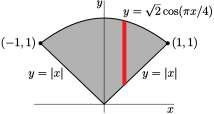
\includegraphics{OE14A_2}
\end{center}

\noindent
Both functions are even, so the region  is symmetric about the $y$--axis.
So, we will compute the area of the part with $x\ge 0$ and multiply
by $2$. The curves $y=\sqrt{2} \cos(\pi x/4)$ and $y=x$ intersect
when $x=\sqrt{2} \cos(\pi x/4)$ or $\cos(\pi x/4)=\frac{x}{\sqrt{2}}$,
which is the case\footnote{The solution $x=1$ was found by guessing.
To guess a solution to $\cos(\pi x/4)=\frac{x}{\sqrt{2}}$ just ask
yourself what simple angle has a cosine that involves $\sqrt{2}$. This
guessing strategy is essentially useless in the real world, but
works great on problem sets and exams.}
when $x=1$. So, using vertical strips as in
the figure above, the area (including the multiplication by 2) is
\begin{equation*}
2\int_0^1 \big[\sqrt{2} \cos(\pi x/4) - x\big]\,\dee{x}
= 2\bigg[\sqrt{2}\,\frac{4}{\pi} \sin(\pi x/4)-\frac{x^2}{2}\bigg]_0^1
= 2\bigg[\frac{4}{\pi}-\frac{1}{2}\bigg] = \frac{8}{\pi}-1
\end{equation*}

\end{solution}
%%%%%%%%%%%%%%%%%%%

\begin{Mquestion}[2016Q2]
Find the area of the finite region that is bounded by the graphs of
$f(x) = x^2\sqrt{x^3+1}$ and $g(x) = 3x^2$.
\end{Mquestion}

\begin{hint}
Figure out where the two curves cross. To determine which curve is above the
other, try evaluating $f(x)$ and $g(x)$ for some simple value of $x$.
Alternatively, consider $x$ very close to zero.
\end{hint}

\begin{answer}
$\dfrac{20}{9}$
\end{answer}

\begin{solution}
For our computation, we will need an antiderivative of
$x^2\sqrt{x^3+1}$, which can be found using the substitution
$u=x^3+1$, $\dee{u} = 3x^2\,\dee{x}$:
\begin{align*}
\int x^2\sqrt{x^3+1} \, \dee{x} = \int \sqrt u \cdot \frac13\,\dee{u} = \frac13\int u^{1/2}\,\dee{u} = \frac13\cdot \frac{u^{3/2}}{3/2}+C = \frac29(x^3+1)^{3/2} + C.
\end{align*}

The two functions $f(x)$ and $g(x)$ are clearly equal at $x=0$. If $x\ne0$, then the functions are equal when
\begin{align*}
3x^2 &= x^2\sqrt{x^3+1} \\
3 &= \sqrt{x^3+1} \\
9 &= x^3+1 \\
8 &= x^3 \\
2 &= x.
\end{align*}
The function $g(x)=3x^2$ is the larger of the two on the interval $[0,2]$, as can be seen by plugging in $x=1$, say, or by observing that when $x$
is very small $f(x)=x^2\sqrt{x^3+1}\approx x^2$ and $g(x)=3x^2$.

\begin{center}
%\begin{tikzpicture}
%\draw[dashed] (4,-0.2) -- (4,6) -- (-0.2,6);
%\draw[domain=0:2.1] plot (2*\x,{\x*\x*sqrt(\x*\x*\x+1)/2});
%\draw[domain=0:2.2] plot (2*\x,{3*\x*\x/2});
%\node[below] at (4,-0.2) {$2$};
%\node[left] at (-0.2,6) {$12$};
%\node at (2,3) {$y=3x^2$};
%\node at (3,0.4) {$y=x^2\sqrt{x^3+1}$};
%\draw[ultra thick,->] (0,0) -- (5,0);
%\draw[ultra thick,->] (0,0) -- (0,8);
%\end{tikzpicture}
     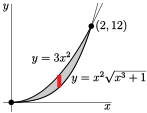
\includegraphics{OQ16_2_4}
\end{center}

The area in question is therefore:
\begin{align*}
\int_0^2 \big( 3x^2 - x^2\sqrt{x^3+1} \big) \, \dee{x} &= \bigg( {x^3} - \frac29(x^3+1)^{3/2} \bigg) \bigg|_0^2 \\
&= \bigg( 2^3 - \frac2 9(2^3+1)^{3/2} \bigg) - \bigg( 0^3 - \frac29(0^3+1)^{3/2} \bigg) \\
&= \bigg( 8 - 6 \bigg) - \bigg( 0 - \frac 2 9 \bigg) =\frac{20}9.
\end{align*}
\end{solution}
%%%%%%%%%%%%%%%%%%%

\begin{Mquestion}[2016Q2]
Find the area to the left of the $y$--axis and to
the right of the curve $x=y^2+y$.
\end{Mquestion}

\begin{hint}
Think about whether it will easier to use vertical strips or horizontal strips.
\end{hint}

\begin{answer}
$\dfrac{1}{6}$
\end{answer}

\begin{solution}
First, let's figure out what our curve $x=y^2+y=y(y+1)$ looks like.
\begin{itemize}
\item The curve intercepts the $y$-axis when $y=0$ and $y=-1$.
\item The $x$-values of the curve are negative when $-1<y<0$, and  positive elsewhere.
\end{itemize}
 This leads to the figure below. We're evaluating the area from $y=-1$ to $y=0$. Since $y^2+y$ is negative there, the length of our (horizontal) slices are $0-(y^2+y)$.

\vspace{0.4in}
\begin{align*}
\text{Area}=\int_{-1}^0\big(0-(y^2+y)\big)\,\dee{y} = -\bigg[\frac{y^3}{3}+\frac{y^2}{2}\bigg]_{-1}^0
=-\frac13+\frac12
=\frac{1}{6}\quad
\smash{\raisebox{-0.33\height}{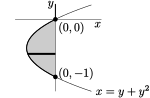
\includegraphics{quiz2M1prob2}}}
\end{align*}
\vspace{0.2in}

\end{solution}
%%%%%%%%%%%%%%%%%%%

\begin{question}
Find the area of the finite region  below $y=\sqrt{9-x^2}$ and above both
 $y=|x|$ and $y=\sqrt{1-x^2}$.
\end{question}
\begin{hint}
Writing an integral for this is nasty. How can you avoid it?
\end{hint}
\begin{answer}
$2\pi$
\end{answer}
\begin{solution}
Let's begin by sketching our region. Note that $y=\sqrt{1-x^2}$ and $y=\sqrt{9-x^2}$ are the top halves of circles centred at the origin with radii 1 and 3, respectively.
\begin{center}
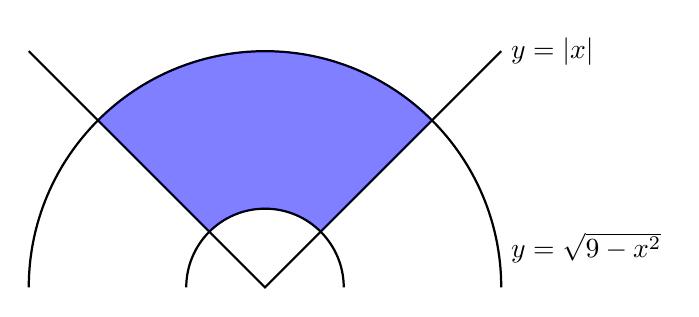
\begin{tikzpicture}
\YEaaxis{4}{4}{1}{4}
\draw[thick] (-3,3)--(0,0)--(3,3);
\draw[thick] (-1,0) arc(180:0:1cm);
\draw[thick] (-3,0) arc(180:0:3cm);
\draw[fill=blue, fill opacity=0.5] (-.71,.71)--(-2.12,2.12) arc(135:45:3) --(.71,.71) arc(45:135:1cm);
\draw (3,.5) node[right] {$y=\sqrt{9-x^2}$};
\draw (3,3) node[right] {$y=|x|$};
\end{tikzpicture}
\end{center}
Our region is the difference of two quarter-circles, so we find its area using geometry:
\[\mbox{Area}=\frac{1}{4}\left(\pi\cdot 3^2\right)-\frac{1}{4}\left(\pi\cdot 1^2\right)=2\pi\]
\end{solution}

%%%%%%%%%%%%%%%%%%%








%%%%%%%%%%%%%%%%%%
\subsection*{\Application}
%%%%%%%%%%%%%%%%%%%

\begin{Mquestion}[2013A]\label{prob_s1.5q5}
The graph below shows the region between
$y = 4 + \pi \sin x$ and $y = 4 + 2\pi - 2x$.

\begin{center}
       \includegraphics{OE13A_4a}
\end{center}

\noindent Find the area of this region.
\end{Mquestion}

\begin{hint}
You are asked for the area, not the signed area. Be very careful about signs.
\end{hint}

\begin{answer}
$2\Big[\pi-\frac{1}{4}\pi^2\Big]$
\end{answer}

\begin{solution}
We will compute the area by using thin vertical strips, as in
the sketch  below:

\begin{center}
       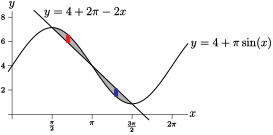
\includegraphics{OE13A_4}
\end{center}

\noindent
By looking at the sketch above, we guess the line $y = 4 + 2\pi - 2x$ intersects the curve
$y = 4 + \pi \sin x$ when $x=\frac{\pi}{2},$ $x=\pi$, and $x=\frac{3\pi}{2}$. Let's make sure these are correct by plugging them into the two equations, and making sure the $y$-values match:

\begin{center}
\begin{tabular}{|c|c|c|c|}
\hline
$x$ & $4+2\pi-2x$ & $4+\pi\sin(x)$ & match?\\[5pt]
\hline
$\frac{\pi}{2}$ & $4+\pi$ & $4+\pi $ & \checkmark\\[5pt]
\hline
$\pi$ & $4$ & $4$ & \checkmark\\[5pt]
\hline
$\frac{3\pi}{2}$ & $4-\pi$ & $4-\pi $ & \checkmark\\[5pt]
\hline
\end{tabular}
\end{center}
Also from
the sketch, we see that:
\begin{itemize}
\item
When $\frac{\pi}{2} \le x \le \pi$, the top of the strip is at
$y = 4 + \pi \sin x$ and the bottom of the strip is at $y = 4 + 2\pi - 2x$.
So the strip has height $\big[(4 + \pi \sin x)-(4 + 2\pi - 2x)\big]$
and width $\dee{x}$, and hence area
$\big[(4 + \pi \sin x)-(4 + 2\pi - 2x)\big]\dee{x}$.

\item
When $\pi \le x \le \frac{3\pi}{2}$, the top of the strip is at
$y = 4 + 2\pi - 2x$ and the bottom of the strip is at $y = 4 + \pi \sin x$.
So the strip has height $\big[(4 + 2\pi - 2x)-(4 + \pi \sin x)\big]$
and width $\dee{x}$, and hence area
$\big[(4 + 2\pi - 2x)-(4 + \pi \sin x)\big]\dee{x}$.
\end{itemize}
Now we can calculate:
\begin{align*}
\hbox{Area}
&= \int_{\pi/2}^\pi \big[(4 + \pi \sin x)-(4 + 2\pi - 2x)\big]\ \dee{x}
   +\int^{3\pi/2}_\pi \big[(4 + 2\pi - 2x)-(4 + \pi \sin x)\big]\ \dee{x}\\
&= \int_{\pi/2}^\pi \big[\pi \sin x- 2\pi + 2x\big]\ \dee{x}
   +\int^{3\pi/2}_\pi \big[2\pi - 2x- \pi \sin x\big]\ \dee{x}\\
&=\Big[-\pi \cos x- 2\pi x + x^2\Big]_{\pi/2}^\pi
  +\Big[2\pi x - x^2+ \pi \cos x\Big]^{3\pi/2}_\pi\\
&=\left[\pi-\pi^2+\frac{3}{4}\pi^2\right]
  +\left[\pi^2-\frac{5}{4}\pi^2+\pi\right]\\
&=2\Big[\pi-\frac{1}{4}\pi^2\Big]
\end{align*}
\end{solution}
%%%%%%%%%%%%%%%%%%%


\begin{question}[1998A]
Compute the area of the finite region bounded by the
curves $x=0$, $x=3$, $y=x+2$ and $y=x^2$.
\end{question}

\begin{hint}
You are asked for the area, not the signed area. Draw a sketch of the region
and be very careful about signs.
\end{hint}

\begin{answer}
$\dfrac{31}{6}$
\end{answer}

\begin{solution}
First, here is a sketch of the region. We are not asked for it, but it
is crucial for understanding the question.
\begin{center}
       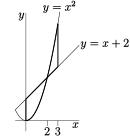
\includegraphics{graphE98A_3}
\end{center}
The two curves  $y=x+2$ and $y=x^2$ cross at $(2,4)$.
The area of the part between them with $0\le x\le 2$ is:
\begin{align*}
\int_0^2 \big[x+2-x^2\big]\,\dee{x}=\Big[\frac{1}{2} x^2+2x-\frac{1}{3}x^3\Big]_0^2
=2+4-\frac{8}{3}=\frac{10}{3}
\end{align*}
The area of the part between the two curves with $2\le x\le 3$ is:
\begin{align*}
\int_2^3 \big[x^2-(x+2)\big]\,\dee{x}=\Big[\frac{1}{3}x^3-\frac{1}{2} x^2-2x\Big]_2^3
=9-\frac{9}{2}-6-\frac{8}{3}+2+4=\frac{11}{6}
\end{align*}
The total area is $\dfrac{10}{3}+\dfrac{11}{6}=\dfrac{31}{6}$.

\end{solution}
%%%%%%%%%%%%%%%%%%%

\begin{question}[2016Q2]
Find the total area between the curves $y = x \sqrt{25-x^2}$ and $y=3x$, on the interval $0\le x\le 4$.
\end{question}

\begin{hint}
You have to determine whether
\begin{itemize}
\item
   the curve $y = f(x) = x \sqrt{25-x^2}$ lies above the line $y=g(x)=3x$ for all          $0\le x\le 4$ or
\item
the curve $y = f(x)$ lies below the line $y=g(x)$ for all $0\le x\le 4$ or
\item  $y=f(x)$ and $y=g(x)$ cross somewhere between $x=0$ and $x=4$.
\end{itemize}
One way to do so is to study the sign of
      $f(x)-g(x) = x\big(\sqrt{25-x^2}-3\big)$.
\end{hint}

\begin{answer}
$\dfrac{26}{3}$
\end{answer}

\begin{solution}
We need to figure out which curve is on top, when. To do this, set $h(x) = 3x - x\sqrt{25-x^2}$. If $h(x) > 0$, then $y=3x$ is the top curve; if $h(x)<0$, then $y=x\sqrt{25-x^2}$ is the top curve.
\begin{align*}
h(x) &= 3x - x\sqrt{25-x^2} = x\left[3-\sqrt{25-x^2}\right]
\intertext{We only care about values of $x$ in $[0,4]$, so $x$ is nonnegative. Then $h(x)$ is positive when:}
3&> \sqrt{25-x^2}\\
9&> 25-x^2\\
x^2 & > 16\\
x&> 4
\end{align*}


That is, $h(x)$ is never positive over the interval $[0,4]$. So, $y = x \sqrt{25-x^2}$ lies above $y=3x$ for all $0\le x\le 4$.

The area we need to calculate is therefore:
\begin{align*}
A &= \int_0^4 \left[x \sqrt{25-x^2} - 3x\right]\,\dee{x} \\
&= \int_0^4 x \sqrt{25-x^2}\,\dee{x} - \int_0^4 3x\,\dee{x} \\&= A_1 - A_2.
\end{align*}
To evaluate $A_1$, we use the substitution
$u(x) = 25-x^2$, for which $\dee{u} = u'(x)\,\dee{x}= -2x\,\dee{x}$;
and $u(4)=25-4^2=9$ when $x=4$,
while $u(0)=25-0^2=25$ when $x=0$. Therefore
\begin{align*}
A_1 &= \int_{x=0}^{x=4} x \sqrt{25-x^2}\,\dee{x}
= -\frac{1}{2} \int_{u=25}^{u=9} \sqrt{u}\,\dee{u}
= \left[-\frac{1}{3} u^{3/2} \right]_{25}^{9}
= \frac{125 - 27}{3} = \frac{98}{3}
\end{align*}
For $A_2$ we use the antiderivative directly:
\begin{equation*}
A_2 = \int_0^4 3x\,\dee{x} =\left[ \frac{3x^2}{2} \right]_0^4 = 24
\end{equation*}
Therefore the total area is:
\begin{align*}
A = \frac{98}{3} - 24 = \frac{26}{3}
\end{align*}

\end{solution}
%%%%%%%%%%%%%%%%%%%

%%%%%%%%%%%%%%%%%%


\begin{question}
Find the area of the finite region below $y=\sqrt{9-x^2}$ and $y=x$, and above  $y=\sqrt{1-(x-1)^2}$.
\end{question}
\begin{hint}
Flex those geometry muscles.
\end{hint}
\begin{answer}
$\dfrac{7\pi}{8}-\dfrac{1}{2}$
\end{answer}
\begin{solution}
Let's begin by sketching our region. Note that $y=\sqrt{9-x^2}$ is the top half of a circle centred at the origin with radius 3, while $y=\sqrt{1-(x-1)^2}$ is the top half of a circle of radius 1 centred at $(1,0)$.
\begin{center}
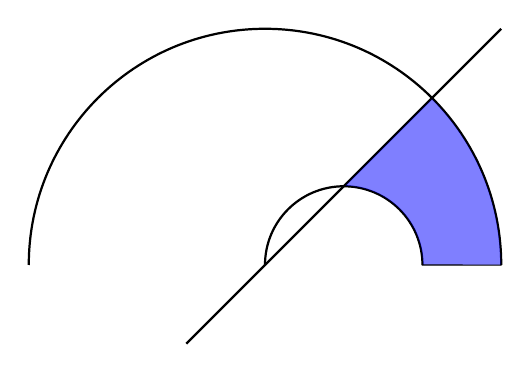
\begin{tikzpicture}
\YEaaxis{4}{4}{1}{4}
\draw[thick] (-1,-1)--(0,0)--(3,3);
\draw[thick] (0,0) arc(180:0:1cm);
\draw[thick] (-3,0) arc(180:0:3cm);
\draw[fill=blue, fill opacity=0.5] (2.12,2.12) arc(45:0:3cm)--(2,0) arc(0:90:1) --cycle ;
\end{tikzpicture}
\end{center}

Note $y=x$ intersects $y=\sqrt{1-(x-1)^2}$ at $(1,1)$, the highest part of the smaller half-circle.

We can easily take the area of  triangles and sectors of circles. With that in mind, we cut up our region the following way:

\begin{center}
\begin{tikzpicture}
\YEaaxis{4}{4}{1}{4}
\draw[thick] (-1,-1)--(0,0)--(3,3);
\draw[thick] (0,0) arc(180:0:1cm);
\draw[thick] (-3,0) arc(180:0:3cm);
\draw[thick, dashed, red, fill=red, fill opacity=0.5] (0,0)--(1,1)|-cycle;
\draw[red] (.5,-.25) node{$A_1$};
\draw[thick, dashed, green, fill=green, fill opacity=0.5] (1,0) --(1,1)arc(90:0:1cm)--cycle;
\draw[green] (1.5,-.25) node{$A_2$};
\draw[blue, ultra thick, fill opacity=0.5, pattern=crosshatch, pattern color=blue] (0,0)--(2.12,2.12) arc(45:0:3cm)--cycle;
\draw[blue] (3.5,1) node{$A_3$};
\end{tikzpicture}
\end{center}
\begin{itemize}
\item The desired area is $A_3-(A_1+A_2)$.
\item $A_1$ is the area of right a triangle with base 1 and height 1, so $A_1 = \frac{1}{2}$.
\item $A_2$ is the area of a quarter circle of radius 1, so $A_2=\frac{\pi}{4}$.
\item $A_3$ is the area of an eighth of a circle of radius 3, so $A_2 = \frac{9\pi}{8}$
\end{itemize}
So, the area of our region is~~ $\dfrac{9\pi}{8} - \dfrac{1}{2}-\dfrac{\pi}{4}=\dfrac{7\pi}{8}-\dfrac{1}{2}$.
\end{solution}

%%%%%%%%%%%%%%%%%%%


\begin{Mquestion}
Find the area of the finite region bounded by the curve $y=x(x^2-4)$ and the line $y=x-2$.
\end{Mquestion}
\begin{hint}
These two functions have three points of intersection. This question is slightly messy, but uses the same concepts we've been practicing so far.
\end{hint}
\begin{answer}
$12\sqrt{2}-\dfrac{13}{4}$
\end{answer}
\begin{solution}
The first function is a cubic, with intercepts at $x=0,\pm2$. The second is a straight line  with a positive slope.

We need to figure out what these functions look like in relation to one another, so let's find their points of intersection.
\begin{align*}
x(x^2-4)&=x-2\\
x(x+2)(x-2)&=x-2\\
\boxed{\color{blue}x-2=0} \quad\mbox{or}\quad x(x+2)&=1\\
x^2+2x-1&=0\\
x &= \dfrac{-2\pm\sqrt{4-4(1)(-1)}}{2}\\
x&=\boxed{\color{red}-1\pm \sqrt{2}}
\end{align*}
So, our three points of intersection are when {\color{blue}$x=2$} and when ${\color{red}x=-1\pm\sqrt{2}}$. We note \[\textcolor{red}{-1-\sqrt{2}} <\textcolor{red}{ -1+\sqrt{2} }< -1+\sqrt{4}<\textcolor{blue}{2}\ .\] So, we need to see which function is on top over the two intervals $\left[-1-\sqrt{2},-1+\sqrt{2}\right]$ and $\left[-1+\sqrt{2},2\right]$. It suffices to check points in these intervals.

\begin{center}
\begin{tabular}{|c|c|c|c|}
\hline
$x$&$x(x^2-4)$ & $x-2$ & top function:\\
\hline
0 & 0 & $-2$ & $x(x^2-4)$\\
\hline
1 & -3 & $-1$ & $x-2$\\
\hline
\end{tabular}
\end{center}


Since 0 is in the interval $\left[-1-\sqrt{2},-1+\sqrt{2}\right]$, $x(x^2-4)$ is the top function in that interval.
Since 1 is in the interval $\left[-1+\sqrt{2},2\right]$, $x-2$ is the top function in that interval. Now we can set up the integral to evaluate the area:
\begin{alignat*}{3}
\mbox{Area}&=\int_{-1-\sqrt{2}}^{-1+\sqrt{2}}\left[x(x^2-4) - (x-2)\right]\ \dee{x}  \quad&&+ \quad
&&\int_{-1+\sqrt{2}}^{2}\left[(x-2)-x(x^2-4)\right]\ \dee{x}\\
&=\int_{-1-\sqrt{2}}^{-1+\sqrt{2}}\left[x^3-5x+2\right]\ \dee{x}  \quad&&+ \quad
&&\int_{-1+\sqrt{2}}^{2}\left[-x^3+5x-2\right]\ \dee{x}
\\&=\left[\frac{1}{4}x^4 - \frac{5}{2}x^2+2x\right]_{-1-\sqrt{2}}^{-1+\sqrt{2}}  \quad&&+ \quad
&&\left[-\frac{1}{4}x^4 + \frac{5}{2}x^2-2x\right]_{-1+\sqrt{2}}^{2}
\intertext{After some taxing but rudimentary algebra:}
&=\left(8\sqrt{2}\right)+\left(4\sqrt{2}-\frac{13}{4}\right)=12\sqrt{2}-\frac{13}{4}
\end{alignat*}
\end{solution}
%%%%%%%%%%%%%%%%%%%
